%
% Copyright (c) 2006-2007 XenSource, Inc.
%
% All rights reserved.
%
% Authors: Ewan Mellor, Richard Sharp, Dave Scott, Jon Harrop.
%

\section{VM Lifecycle}

\begin{figure}
\centering
\resizebox{0.9\textwidth}{!}{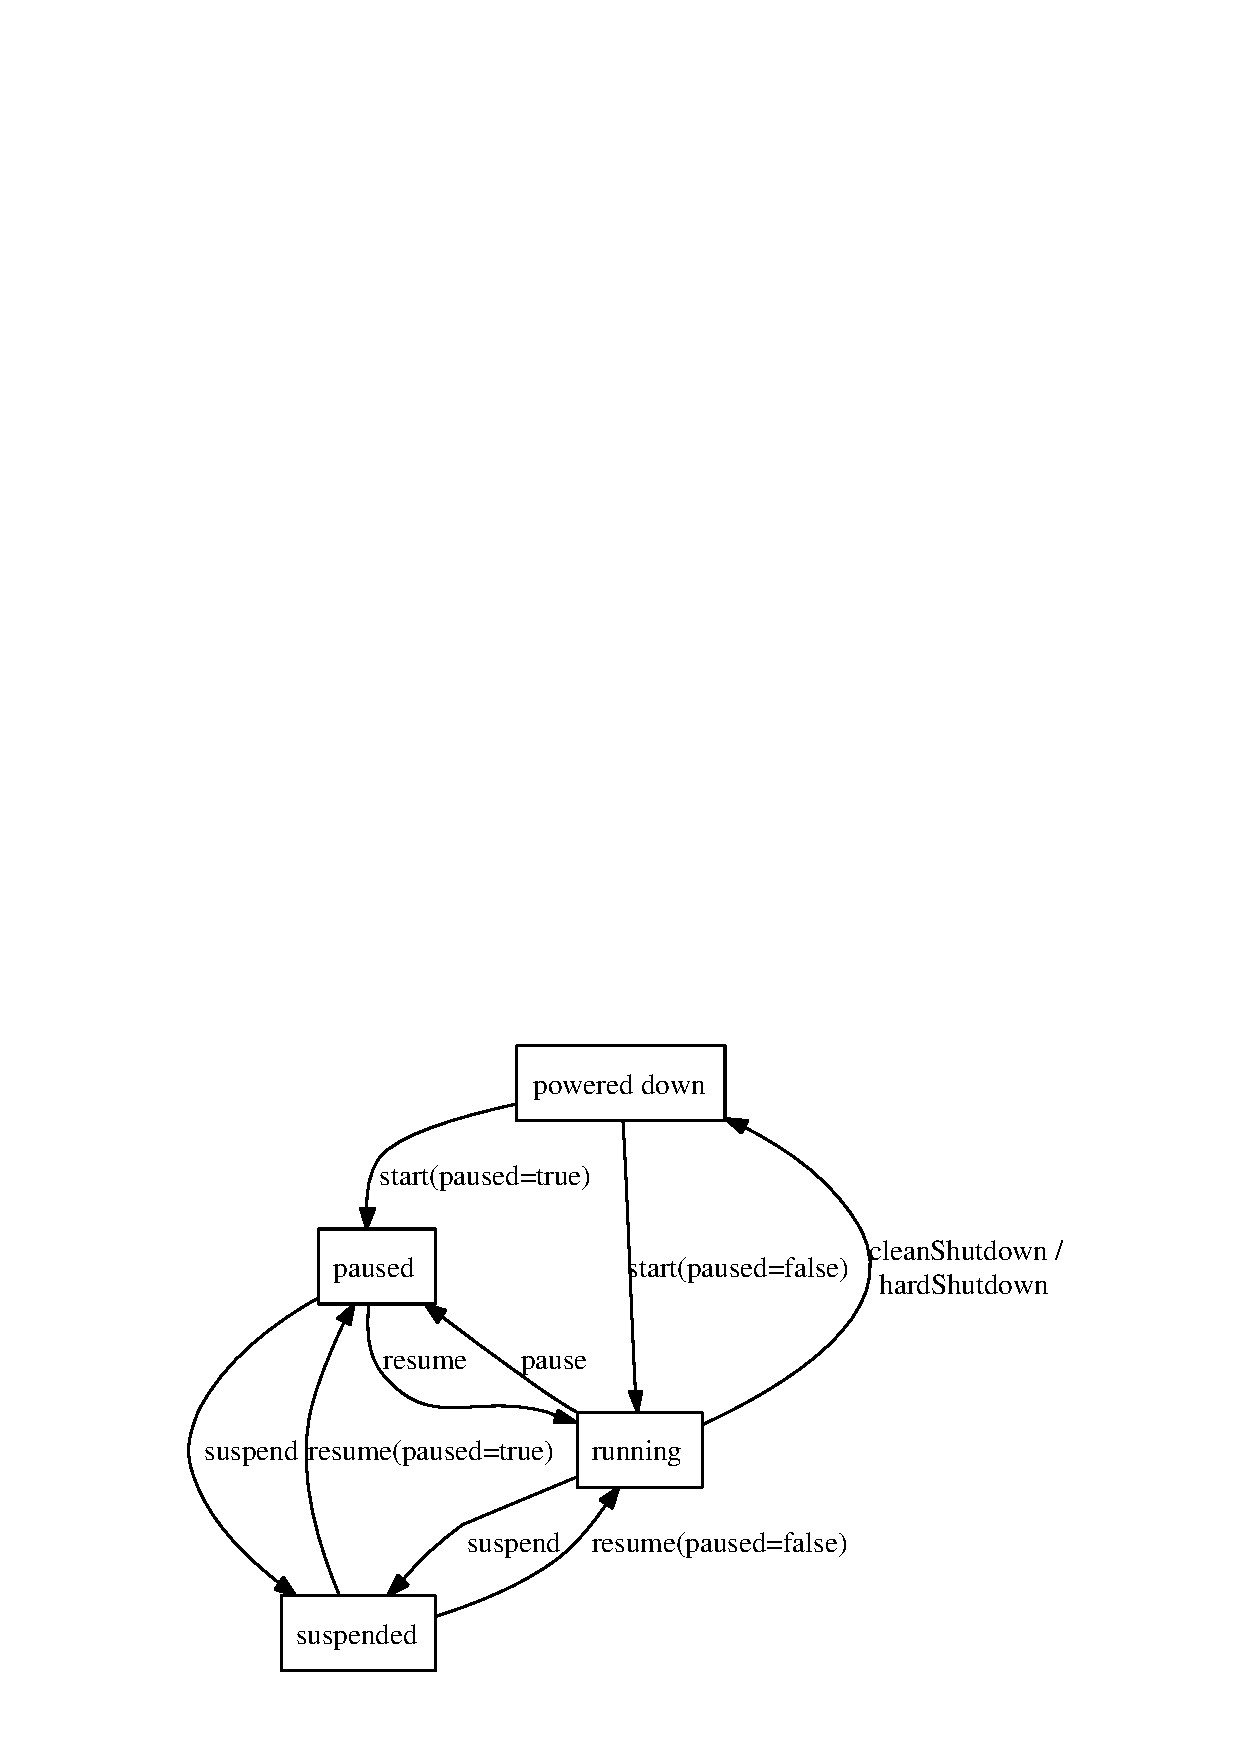
\includegraphics{vm_lifecycle}}
\caption{VM Lifecycle}
\label{fig-vm-lifecycle}
\end{figure}

Figure~\ref{fig-vm-lifecycle} shows the states that a VM can be in
and the API calls that can be used to move the VM between these states.

\section{VM boot parameters}

The VM class contains a number of fields that control the way in which the VM is booted.
With reference to the fields defined in the VM class (see later in this document),
this section outlines the boot options available and the mechanisms provided for controlling them.

VM booting is controlled by setting one of the two mutually exclusive groups: ``PV'', and ``HVM''.  If HVM.boot\_policy is the empty string, then paravirtual domain building and booting will be used; otherwise the VM will be loaded as an HVM domain, and booted using an emulated BIOS.

When paravirtual booting is in use, the PV/bootloader field indicates the bootloader to use.  It may be ``pygrub'', in which case the platform's default installation of pygrub will be used, or a full path within the control domain to some other bootloader.  The other fields, PV/kernel, PV/ramdisk, PV/args and PV/bootloader\_args will be passed to the bootloader unmodified, and interpretation of those fields is then specific to the bootloader itself, including the possibility that the bootloader will ignore some or all of those given values. Finally the paths of all bootable disks are added to the bootloader commandline (a disk is bootable if its VBD has the bootable flag set). There may be zero, one or many bootable disks; the bootloader decides which disk (if any) to boot from.

If the bootloader is pygrub, then the menu.lst is parsed if present in the guest's filesystem, otherwise the specified kernel and ramdisk are used, or an autodetected kernel is used if nothing is specified and autodetection is possible.  PV/args is appended to the kernel command line, no matter which mechanism is used for finding the kernel.

If PV/bootloader is empty but PV/kernel is specified, then the kernel and ramdisk values will be treated as paths within the control domain.  If both PV/bootloader and PV/kernel are empty, then the behaviour is as if PV/bootloader was specified as ``pygrub''.

When using HVM booting, HVM/boot\_policy and HVM/boot\_params specify the boot handling.  Only one policy is currently defined: ``BIOS order''.  In this case, HVM/boot\_params should contain one key-value pair ``order'' = ``N'' where N is the string that will be passed to QEMU.